% The governing equation, for contemplation: derivation on one side, geometry on the other,
% with the actual angular shape of D_ab drawn.  Compile: pdflatex -interaction=nonstopmode
\documentclass[border=16pt]{standalone}
\usepackage{amsmath}
\usepackage{tikz}
\usetikzlibrary{positioning,arrows.meta,calc,backgrounds}

\definecolor{ink}{RGB}{45,55,70}
\definecolor{cLaw}{RGB}{238,240,244}
\definecolor{tSrc}{RGB}{42,84,140}
\definecolor{tFind}{RGB}{40,110,55}
\definecolor{tNeg}{RGB}{170,55,55}
\definecolor{note}{RGB}{105,105,115}

\begin{document}
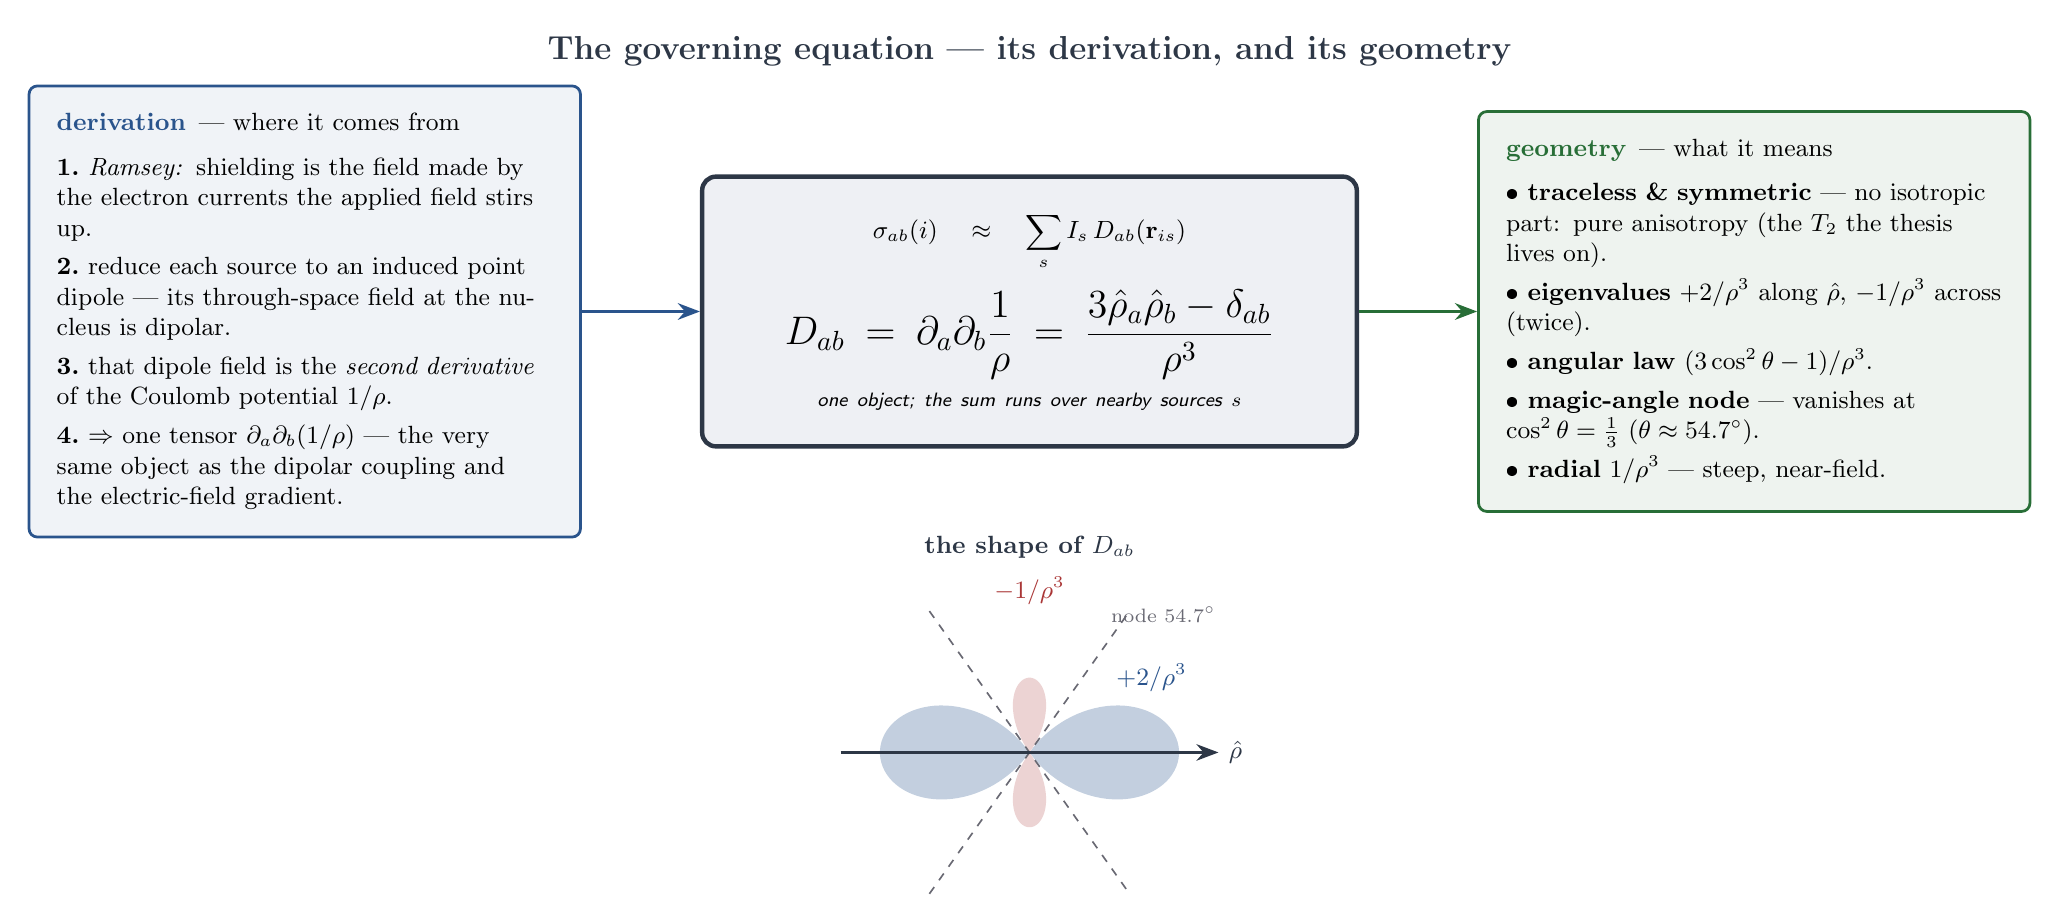
\begin{tikzpicture}[
  font=\sffamily,
  >={Stealth[length=2.8mm]},
  ceq/.style={rounded corners=5pt, draw=ink, line width=1.6pt, fill=cLaw, align=center, inner sep=13pt},
  der/.style={rounded corners=3pt, draw=tSrc, line width=1pt, fill=tSrc!7, align=left, inner sep=10pt, text width=6.3cm, font=\small},
  geo/.style={rounded corners=3pt, draw=tFind, line width=1pt, fill=tFind!8, align=left, inner sep=10pt, text width=6.3cm, font=\small},
]

% ---- title ----
\node[font=\large\bfseries, text=ink] (T) at (0,4.9) {The governing equation --- its derivation, and its geometry};

% ---- centre: the kernel ----
\node[ceq, text width=7.4cm] (CEQ) at (0,1.6) {%
  {\small $\displaystyle \sigma_{ab}(i)\ \approx\ \sum_s I_s\,D_{ab}(\mathbf r_{is})$}\\[6pt]
  {\Large $\displaystyle D_{ab}=\partial_a\partial_b\frac{1}{\rho}=\frac{3\hat\rho_a\hat\rho_b-\delta_{ab}}{\rho^{3}}$}\\[4pt]
  {\scriptsize\itshape one object; the sum runs over nearby sources $s$}};

% ---- derivation (left) ----
\node[der, left=1.5cm of CEQ] (DER) {%
  \textbf{\textcolor{tSrc}{derivation}}\, --- where it comes from\\[5pt]
  \textbf{1.}\ \emph{Ramsey:} shielding is the field made by the electron currents the applied field stirs up.\\[3pt]
  \textbf{2.}\ reduce each source to an induced point dipole --- its through-space field at the nucleus is dipolar.\\[3pt]
  \textbf{3.}\ that dipole field is the \emph{second derivative} of the Coulomb potential $1/\rho$.\\[3pt]
  \textbf{4.}\ $\Rightarrow$ one tensor $\partial_a\partial_b(1/\rho)$ --- the very same object as the dipolar coupling and the electric-field gradient.};

% ---- geometry (right) ----
\node[geo, right=1.5cm of CEQ] (GEO) {%
  \textbf{\textcolor{tFind}{geometry}}\, --- what it means\\[5pt]
  \textbullet\ \textbf{traceless \& symmetric} --- no isotropic part: pure anisotropy (the $T_2$ the thesis lives on).\\[3pt]
  \textbullet\ \textbf{eigenvalues} $+2/\rho^3$ along $\hat\rho$, $-1/\rho^3$ across (twice).\\[3pt]
  \textbullet\ \textbf{angular law} $(3\cos^2\theta-1)/\rho^3$.\\[3pt]
  \textbullet\ \textbf{magic-angle node} --- vanishes at $\cos^2\theta=\tfrac13$ ($\theta\approx 54.7^\circ$).\\[3pt]
  \textbullet\ \textbf{radial} $1/\rho^3$ --- steep, near-field.};

% ---- arrows ----
\draw[->, line width=1.3pt, tSrc] (DER.east) -- (CEQ.west);
\draw[->, line width=1.3pt, tFind] (CEQ.east) -- (GEO.west);

% ---- the actual angular shape of D_ab ----
\node[font=\small\bfseries, text=ink] at (0,-1.4) {the shape of $D_{ab}$};
\begin{scope}[shift={(0,-4.0)}]
  % positive lobes (within 54.7deg of the rho-hat axis)
  \fill[tSrc!28] plot[domain=-54.7:54.7,samples=70] (\x:{0.95*abs(3*cos(\x)*cos(\x)-1)}) -- cycle;
  \fill[tSrc!28] plot[domain=125.3:234.7,samples=70] (\x:{0.95*abs(3*cos(\x)*cos(\x)-1)}) -- cycle;
  % negative belt (around the equator)
  \fill[tNeg!22] plot[domain=54.7:125.3,samples=50] (\x:{0.95*abs(3*cos(\x)*cos(\x)-1)}) -- cycle;
  \fill[tNeg!22] plot[domain=234.7:305.3,samples=50] (\x:{0.95*abs(3*cos(\x)*cos(\x)-1)}) -- cycle;
  % magic-angle nodes
  \draw[dashed, note, line width=0.6pt] (234.7:2.2)--(0,0)--(54.7:2.2);
  \draw[dashed, note, line width=0.6pt] (125.3:2.2)--(0,0)--(-54.7:2.2);
  % the rho-hat axis
  \draw[->, ink, line width=0.9pt] (-2.4,0)--(2.4,0) node[right, font=\small]{$\hat\rho$};
  % labels
  \node[font=\small, tSrc] at (1.55,0.95) {$+2/\rho^3$};
  \node[font=\small, tNeg] at (0,2.05) {$-1/\rho^3$};
  \node[font=\scriptsize, note] at (1.7,1.75) {node $54.7^\circ$};
\end{scope}

\end{tikzpicture}
\end{document}
